\documentclass[a4paper]{article}
\usepackage{fancyhdr}
\usepackage{enumitem}
\usepackage{tikz}
\usepackage{float} \usepackage{listings}

\title{Homework module \#2: Compiler Technology}

\lhead{Homework module \#2}
\rhead{TDT4205 - Compilers}

\author{Aleksander Vognild Burkow}

\lstset{
    language=C,
    tabsize=2,
    frame=single
}

\begin{document}

\maketitle
\thispagestyle{empty}
\newpage

\part{Theory}
\section{Regular languages}

\begin{enumerate}[label=\alph*)]
\item
    The following is a NFA implementation of the regular expression. \ref{fig:nfa}
    \begin{center}
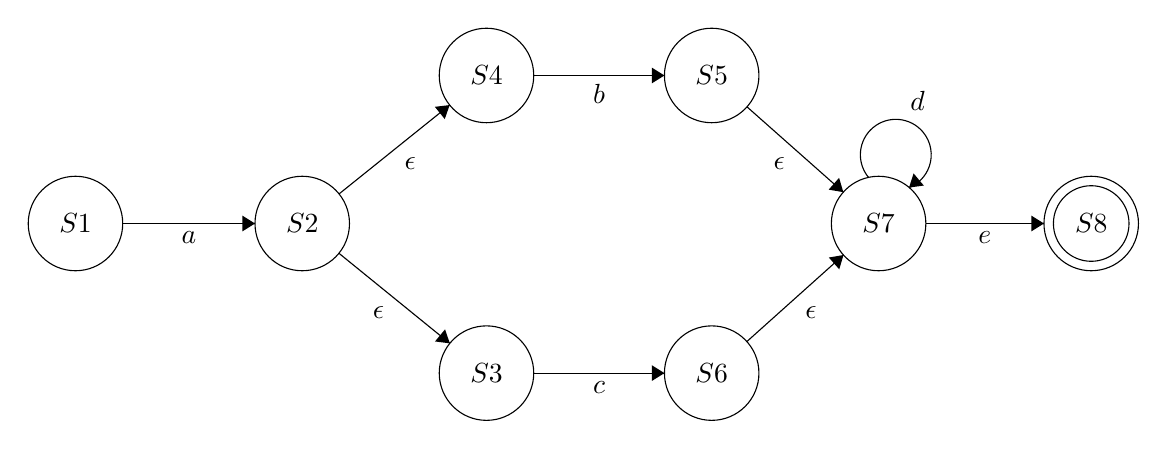
\begin{tikzpicture}[scale=0.2]
\tikzstyle{every node}+=[inner sep=0pt]
\draw [black] (8.1,-31) circle (3);
\draw (8.1,-31) node {$S1$};
\draw [black] (22.5,-31) circle (3);
\draw (22.5,-31) node {$S2$};
\draw [black] (34.2,-40.5) circle (3);
\draw (34.2,-40.5) node {$S3$};
\draw [black] (34.2,-21.6) circle (3);
\draw (34.2,-21.6) node {$S4$};
\draw [black] (48.5,-21.6) circle (3);
\draw (48.5,-21.6) node {$S5$};
\draw [black] (48.5,-40.5) circle (3);
\draw (48.5,-40.5) node {$S6$};
\draw [black] (59.1,-31) circle (3);
\draw (59.1,-31) node {$S7$};
\draw [black] (72.6,-31) circle (3);
\draw (72.6,-31) node {$S8$};
\draw [black] (72.6,-31) circle (2.4);
\draw [black] (11.1,-31) -- (19.5,-31);
\fill [black] (19.5,-31) -- (18.7,-30.5) -- (18.7,-31.5);
\draw (15.3,-31.5) node [below] {$a$};
\draw [black] (24.84,-29.12) -- (31.86,-23.48);
\fill [black] (31.86,-23.48) -- (30.92,-23.59) -- (31.55,-24.37);
\draw (29.36,-26.79) node [below] {$\epsilon$};
\draw [black] (24.83,-32.89) -- (31.87,-38.61);
\fill [black] (31.87,-38.61) -- (31.57,-37.72) -- (30.93,-38.49);
\draw (27.34,-36.24) node [below] {$\epsilon$};
\draw [black] (37.2,-40.5) -- (45.5,-40.5);
\fill [black] (45.5,-40.5) -- (44.7,-40) -- (44.7,-41);
\draw (41.35,-41) node [below] {$c$};
\draw [black] (37.2,-21.6) -- (45.5,-21.6);
\fill [black] (45.5,-21.6) -- (44.7,-21.1) -- (44.7,-22.1);
\draw (41.35,-22.1) node [below] {$b$};
\draw [black] (50.74,-23.59) -- (56.86,-29.01);
\fill [black] (56.86,-29.01) -- (56.59,-28.1) -- (55.93,-28.85);
\draw (52.79,-26.79) node [below] {$\epsilon$};
\draw [black] (58.467,-28.08) arc (219.96376:-68.03624:2.25);
\draw (61.57,-23.87) node [above] {$d$};
\fill [black] (61.03,-28.72) -- (61.97,-28.59) -- (61.32,-27.82);
\draw [black] (62.1,-31) -- (69.6,-31);
\fill [black] (69.6,-31) -- (68.8,-30.5) -- (68.8,-31.5);
\draw (65.85,-31.5) node [below] {$e$};
\draw [black] (50.73,-38.5) -- (56.87,-33);
\fill [black] (56.87,-33) -- (55.94,-33.16) -- (56.6,-33.91);
\draw (54.81,-36.24) node [below] {$\epsilon$};
\end{tikzpicture}
\end{center}


\item
    The converted NFA is presented below. \ref{fig:dfa}
    \begin{figure}[H]
\begin{center}
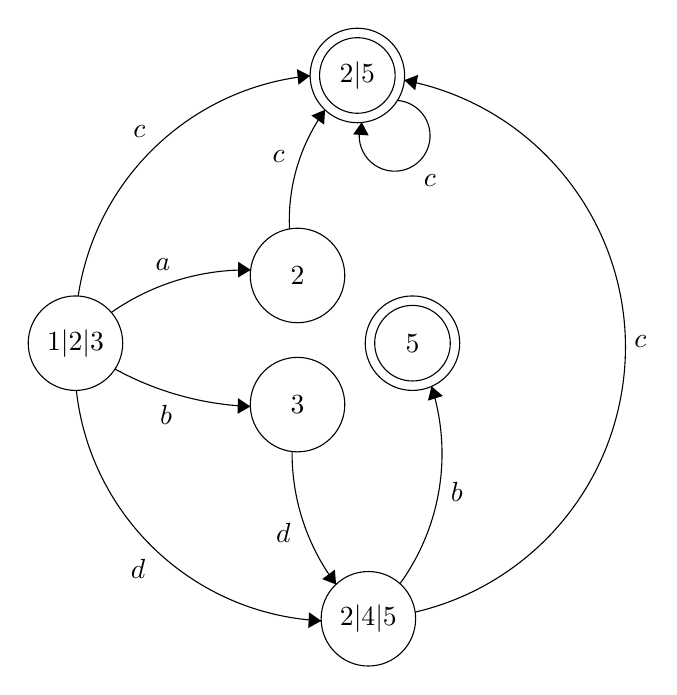
\begin{tikzpicture}[scale=0.2]
\tikzstyle{every node}+=[inner sep=0pt]
\draw [black] (20.4,-29.4) circle (3);
\draw (20.4,-29.4) node {$1|2|3$};
\draw [black] (39,-46.9) circle (3);
\draw (39,-46.9) node {$2|4|5$};
\draw [black] (38.3,-12.4) circle (3);
\draw (38.3,-12.4) node {$2|5$};
\draw [black] (38.3,-12.4) circle (2.4);
\draw [black] (34.5,-25.1) circle (3);
\draw (34.5,-25.1) node {$2$};
\draw [black] (34.5,-33.3) circle (3);
\draw (34.5,-33.3) node {$3$};
\draw [black] (41.8,-29.4) circle (3);
\draw (41.8,-29.4) node {$5$};
\draw [black] (41.8,-29.4) circle (2.4);
\draw [black] (36.007,-47.028) arc (-92.78149:-173.72788:16.449);
\fill [black] (36.01,-47.03) -- (35.23,-46.49) -- (35.18,-47.49);
\draw (24.37,-43.06) node [below] {$d$};
\draw [black] (20.571,-26.409) arc (-188.47934:-264.47509:16.502);
\fill [black] (35.3,-12.42) -- (34.46,-12) -- (34.56,-12.99);
\draw (24.46,-16.39) node [above] {$c$};
\draw [black] (40.834,-13.984) arc (85.72034:-202.27966:2.25);
\draw (42.9,-18.64) node [below] {$c$};
\fill [black] (38.58,-15.37) -- (38.03,-16.14) -- (39.02,-16.21);
\draw [black] (31.505,-33.418) arc (-92.17099:-118.75145:19.401);
\fill [black] (31.51,-33.42) -- (30.72,-32.89) -- (30.69,-33.89);
\draw (26.16,-33.3) node [below] {$b$};
\draw [black] (22.672,-27.449) arc (124.92445:88.99524:15.005);
\fill [black] (31.53,-24.75) -- (30.73,-24.23) -- (30.72,-25.23);
\draw (25.96,-24.85) node [above] {$a$};
\draw [black] (41.281,-12.702) arc (79.23965:-76.91492:17.264);
\fill [black] (41.28,-12.7) -- (41.97,-13.34) -- (42.16,-12.36);
\draw (55.85,-29.31) node [right] {$c$};
\draw [black] (43.009,-32.139) arc (17.70557:-35.88613:14.079);
\fill [black] (43.01,-32.14) -- (42.78,-33.05) -- (43.73,-32.75);
\draw (44.21,-38.86) node [right] {$b$};
\draw [black] (36.948,-44.719) arc (-142.95292:-180.43014:13.845);
\fill [black] (36.95,-44.72) -- (36.87,-43.78) -- (36.07,-44.38);
\draw (34.09,-41.42) node [left] {$d$};
\draw [black] (33.99,-22.152) arc (-177.37009:-215.9456:11.958);
\fill [black] (36.25,-14.58) -- (35.38,-14.94) -- (36.19,-15.52);
\draw (33.71,-17.57) node [left] {$c$};
\end{tikzpicture}
\caption{DFA}
\label{fig:dfa}
\end{center}
\end{figure}


\newpage
\item
    The program will be able to remove simple while loops without any nesting inside.

    Issues will arise in the following cases:
    \begin{enumerate}[label=\roman*]
    \item
    Nested statements:

\begin{lstlisting}
while (COND) {
    if (1) {
    } // End will be matched
}
\end{lstlisting}

    Flex will match the end of the while with the end of the if statement.

    \item
    Do while constructs:
\begin{lstlisting}
do {
    ...
} while (COND);
if (3.14) {
    // Will be matched here
}
\end{lstlisting}

    The end of the do while statement be matched with the end if the if. The do part remains intact.

    \item
    Strings:

\begin{lstlisting}
while (true) {
    char omfg[] = "do not touch my while {";
}
\end{lstlisting}

    Flex will mistakenly demolish the string.
    \end{enumerate}

The correct way to remove loops would be to ignore the node at the parser level. The lexer has no idea about the semantic meanings of the tokens may encounter, and cannot decide if the matched brackets belong to a while statement or some poor soon-to-be dismembered if statement.

Implementing removal of while-loops in bison (by ignoring the node) will ensure only well formed while-loops will be removed.


\end{enumerate}

\newpage

\section{Grammars}

\begin{enumerate}[label=\alph*)]

\item
    An ambigous grammar is a formal grammar which allows for more than one leftmost derivation for any expression.

\item
    Ambiguity is an undecidable problem, but if we study the string $ mvmp $ we see that two productions arise:

\begin{enumerate}[label=\roman*]
\item
    S = NvN  (Use S = NvN)

    NvN = mvN (Use N = m)

    mvN = mvmp (Use N = mp)

    mvmp

\item
    S = Sp (Use S = NvN)

    Sp = NvNp (Use S = NvN)

    NvNp = mvmp (Use N = m)

    mvmp

\end{enumerate}
Here we see two different parse trees for the same production. We conclude the grammar is ambigous.

\item
An left-recursive grammar is a grammar in which there exists a non-terminal where one of its productions (transitive or immediate) has itself as the leftmost symbol.

\item
The grammar is left recursive. This is seen by the fact that we can produce $ Sp $ from $ S $.
    
    

\end{enumerate}


\end{document}
